\documentclass[a4paper, 12pt]{article}
\usepackage{enumitem}
\usepackage[utf8]{inputenc}
\usepackage{graphicx}
\usepackage{fancyhdr}
\usepackage[left=2.5cm, right=2.5cm, top=3cm, bottom=3cm]{geometry}
\graphicspath{{Imagenes/}}

%-------------------------ENCABEZADO Y PIE DE PÁGINA----------------------
\pagestyle{fancy}
\fancyhf{}
\setlength{\headheight}{30 pt}
\renewcommand{\headrulewidth}{0.2pt}
\fancyhead[L]{\begin{tabular}{@{}l@{}}
\includegraphics[scale=0.4]{escudo.PNG}\end{tabular}}
\fancyhead[R]{\begin{tabular}{@{}c@{}} \textbf{Inteligencia Artificial I} \\ Trabajo Final \end{tabular}}



\fancyfoot[L]{\begin{tabular}{@{}l@{}}\includegraphics[scale=0.4]{año.PNG}\end{tabular}}
\fancyfoot[R]{\thepage}
\fancyfoot[C]{\begin{tabular}{@{}c@{}}\textbf{BORQUEZ PEREZ Juan Manuel}\\ \textbf{Legajo 13567}\end{tabular}}
\renewcommand{\footrulewidth}{0.2pt}

\begin{document}
%-----------------------------PÁGINA PRINCCIPAL---------------------------
\begin{titlepage}
    \centering
    \vspace*{5cm}
    {\Large\bfseries Trabajo Final Inteligencia Artificial I - Año 2023}\\
    \vspace{0.2cm}
    {\Large \textbf{Visión Artificial y Reconocimiento de Voz}}\\
    \vspace{0.7cm}
    {\Large Ingeniería en Mecatrónica}\\
    \vspace{1.5cm}
    Alumno: Juan Manuel BORQUEZ PEREZ\\
    Legajo: 13567\\
    \vfill
    {\begin{tabular}{@{}c@{}}
\includegraphics[scale=0.4]{escudo.PNG}\end{tabular}}\hspace{10pt}
    {\begin{tabular}{@{}c@{}}\includegraphics[scale=0.6]{año.PNG}\end{tabular}}
    %Año 2023
\end{titlepage}

\section{Resumen}
%------------------------------------RESUMEN------------------------------
En este informe se presenta el desarrollo de una solución al problema propuesto por la cátedra. Se tiene una máquina expendedora de 4 tipos de fruta: manzana, naranja, banana y pera. La máquina cuenta con una cámara para tomar fotos de las frutas en los estantes y un micrófono para solicitar frutas por voz. El software de la máquina identifica las frutas en las imágenes y sus nombres cuando son mencionadas por el usuario. La clasificación de la voz se realiza mediante un algoritmo \textbf{KNN} con k=3, y la clasificación de las imágenes se lleva a cabo con un algoritmo KNN con k=1 comparando cada imagen con los centroides obtenidos del entrenamiento de un segmentador basado en \textbf{KMeans}. Se construyó un dataset disponible en línea con audios de varias personas e imágenes recopiladas en línea o tomadas por alumnos. Los resultados obtenidos fueron suficientemente satisfactorios; en concreto, la validación del modelo de reconocimiento de voz se realizó con 24 archivos de distintas personas sin falla. El reconocimiento de frutas en imágenes, aunque no completamente probado, es vulnerable ante frutas descoloridas, siendo el color la característica principal para la separación. El desarrollo se encuentra principalmente documentado en notebooks de Jupyter.
\vspace{0.5cm}

This report presents the development of a solution to the problem proposed by the department. There is a vending machine with 4 types of fruit: apple, orange, banana, and pear. The machine is equipped with a camera to take photos of the fruits on the shelves and a microphone to request fruits by voice. The machine's software identifies the fruits in the images and their names when mentioned by the user. Voice classification is done using a KNN algorithm with k=3, and image classification is performed with a KNN algorithm with k=1 comparing each image with centroids obtained from training a KMeans-based segmenter. A dataset, available online, was built with audio from various people and images collected online or taken by students. The results obtained were sufficiently satisfactory; specifically, voice recognition model validation was performed with 24 files from different people without failure. Fruit recognition in images, although not fully tested, is vulnerable to discolored fruits, with color being the main feature for separation. The development is primarily documented in Jupyter notebooks.

\section{Introduccion}
%----------------------------------INTRODUCCION--------------------------
\subsection{Visión Artificial}
La visión artificial es la tecnología que le permite a las equipos industriales percibir las características del entorno a través de imágenes de forma automática. A diferencia de un simple procesamiento de imágenes, en el que el resultado de una imagén de entrada es otra imágen de salida modificada, la visión artificial implica la extracción de características relevantes de las imágenes que permitan identificar los elementos de interés del entorno. Las imágenes se pueden obtener con distintos tipos de sensores y es así que se tienen imágenes como las que se pueden obtener con una camara tradicional sensible a la radiación en el rango del espectro visible o imágenes termográficas obtenidas con sensores sensibles a la radiación infraroja del espectro por dar ejemplos.

La visión artificial clásica es un campo que se comenzó a desarrollar mucho antes del desarrollo de las aplicaciones más avanzadas como el Machine Learning y sin embargo, a través de simples operaciones con características de las imágenes permitió identificar diferentes elementos en principio bien definidos como códigos de barras, bordes, objetos, colores, etc.

Las aplicaciones de la visión artifical son variadas e incluyen la detección de defectos en partes de máquinas, medición de partes, identificación y rastreo de objetos, identificación de textos, etc.
Los principales elementos involucrados en la obtención de imágenes para la visión artificial son: una fuente de luz, un escenario específico y controlado para capturar una toma o un elemento para lograr dicho escenario como un gripper, aumentos y un sensor para capturar la imágen, en general una camará de algún tipo.

En este trabajo se implementa la visión artificial en el sentido clásico para extraer características de imágenes de 4 tipos de frutas: peras, bananas, manzanas y naranjas con el objeto de hacer una segmentación del conjunto de imágenes en grupos según el tipo de fruta.

Inicialmente se planteó la solución al problema tratando de que sea lo suficientemente robusta como para poder identificar las frutas en cualquier tipo de fondo, en ese sentido se exploraron diversas características, máscaras y estrategias para tratar de separar a las frutas del fondo. Sin embargo, el problema de lograr la robustez no se pudo resolver de forma satisfactoria en todos los casos y por falta de tiempo se decidió tomar mayor control del escenario optandose finalmente por el uso de fondo blanco en todos los casos.

Para entrenar el segmentador fue necesario disponer de un dataset de imágenes de entrenamiento. De este dataset, algunas de las imágenes se obtuvieron de recopilación de imágenes en línea mientras que la mayoría se obtuvieron tomando fotos a frutas con la cámara de un celular. En las imágenes capturadas no se tuvo demasiado recaudo en cuanto a la escena más que la utilización de luz natural y el posicionamiento de la fruta en algún fondo blanco.

Se exploraron diversas características de las imágenes como los bordes, texturas, color, etc., que fueron relevantes tanto para la separación de las frutas del fondo como para lograr la posterior segmentación del conjunto de imágenes en grupos de frutas.
\subsection{Reconocimiento de Voz}

El reconocimiento de voz es la capacidad de un sistema de software para transformar el discurso de una persona en su representación en texto, permitiendo la comunicación entre un humano y una computadora a través del habla. Este tipo de sistemas integran diferentes tipos de información contenida en la señal de audio, como la gramática, la sintaxis, la estructura y la composición del audio, incluso en presencia de ambigüedades, incertidumbres y perturbaciones como el ruido, con el objetivo de obtener una interpretación aceptable del mensaje que se desea transmitir. Estos sistemas se utilizan en aplicaciones como el dictado automático, el control por comandos de voz, traductores, reconocimiento de canciones, entre otras.

Este tipo de sistemas pueden utilizar aprendizaje deductivo o sistemas expertos, que son entrenados con los conocimientos de un conjunto de campos involucrados en el habla, tales como la lingüística, la fonética, la acústica, etc. También pueden ser sistemas que hagan uso de aprendizaje inductivo, en el cual el sistema tiene la capacidad de adquirir los conocimientos necesarios de manera automática. Dentro de esta última categoría se encuentran la mayoría de las técnicas utilizadas: Hidden Markov Models, N-Grams y Redes Neuronales.

En el trabajo que se presenta aquí, el reconocimiento del discurso se limita a la identificación de los nombres de las frutas mencionadas. Tanto si se trata de una solución con aprendizaje automático como la solución que se presenta en este caso, en la cual no se utiliza tal técnica, es necesario llevar a cabo la extracción de las características que representan la información relevante contenida en la señal. La parte más complicada de esta solución radica precisamente en el preprocesamiento de las señales de audio para lograr pasar por alto perturbaciones como el silencio o el ruido, y la posterior extracción de características que permitan diferenciar audios de distintas frutas. Después de extraer un conjunto de características que permitan separar adecuadamente el conjunto de audios, la clasificación de un nuevo dato a través del algoritmo k-NN es algo trivial.
%--------------------------------------ESPECIFICACIÓN DEL AGENTE------------------------------------
\section{Especificación del Agente}
\subsection{Descripción y tipo de Agente}

El agente se ha interpretado de la siguiente manera. El mismo consiste en una máquina expendedora de frutas. La máquina dispone de 4 estanterías, en cada una de las cuales se encuentra uno de los tipos de fruta considerados. Cuando un usuario desea obtener una fruta de la máquina expendedora, presiona un botón para hablar en el micrófono de la máquina y decir el nombre de la fruta deseada. El programa del agente le permite identificar el nombre de la fruta mencionada. Luego, el agente determina si la fruta se encuentra en alguna de las estanterías y, si es así, identifica en cuál de las estanterías se encuentra la fruta. Entonces, a través de un actuador empuja la fruta del estante para expenderla al usuario. Para la determinación de la existencia y ubicación de la fruta solicitada, previo al requerimiento del usuario, el agente toma imágenes a través de una cámara de las frutas en los estantes y las clasifica. La actualización de esta información se realiza siempre que la disposición de frutas en los estantes es modificada.

Se considera que se trata de un \textbf{agente que aprende} debido a que los algoritmos que utiliza para la clasificación de las frutas en imágenes y por voz están comprendidos dentro de ese tipo de agentes (\cite{referencia}). El aprendizaje como tal se evidencia sobre todo en el algoritmo K-means, ya que durante el entrenamiento, el agente se vuelve capaz de encontrar similitudes y diferencias entre los grupos de imágenes. Por otro lado, en la clasificación de frutas por voz, no existe una etapa de entrenamiento como tal, y el agente requiere toda la base de datos de audio para hacer una predicción en base a una nueva orden (aprendizaje basado en memoria \cite{referencia}). En ambos casos, se puede decir que el agente tiene la capacidad de mejorar su habilidad para clasificar imágenes y audio mediante la incorporación de más datos a la base de datos de imágenes y audios utilizados para el entrenamiento, razón por la cual se considera como un agente que aprende. En esta implementación, sin embargo, no se contempla la posibilidad de que audios de nuevas órdenes o las nuevas imágenes tomadas de las frutas en la estantería sean incorporadas a la base de entrenamiento para reentrenar al segmentador K-means o para ampliar los datos del clasificador k-NN para audio. Terminada la validación del clasificador de audios y entrenado el segmentador de imágenes, el comportamiento del agente es como el de un \textbf{agente basado en modelos} dado que son los moedelos entrenados que permiten identificar lon nombres y los objetos. En suma, existe durante la propia implementación del agente un proceso de ajuste no automático sino asistido por el diseñador del sistema y en base a una comparación entre el rendimiento que tiene el agente en un instante determinado y el rendimiento esperado.
%------------------------------TABLA-------------------------------
\newpage
\subsection{Tabla REAS}
\begin{table}[htbp]
    \centering
    \begin{tabular}{|p{3.5cm}|p{3.5cm}|p{3.5cm}|p{3.5cm}|}
        \hline
        \textbf{Rendimiento} & \textbf{Entorno} & \textbf{Actuadores} & \textbf{Sensores} \\
        \hline
        \begin{itemize}[left=0pt, itemsep=-2pt]
            \item Exactitud en el reconocimiento de las frutas medida por el número de aciertos respecto del total de ordenes del usuario.
            \item Rapidez en la respuesta del agente medida como el tiempo entre en que el usuario lleva a cabo una orden y recibe la fruta requerida.
            \item Tratamiento cuidadoso de las frutas.
        \end{itemize} & 
        \begin{itemize}[left=0pt, itemsep=-2pt]
            \item El gabinete de la máquina con los estantes, el estado de los mismos y la iluminación.
            \item El entorno en donde la máquina se ubica, su ruido ambiental y la iluminación.
            \item Los usuarios de la máquina.
        \end{itemize} & 
        \begin{itemize}[left=0pt, itemsep=-2pt]
            \item Elementos de manipulación de la cámara para desplazarla y tomar fotos en los estantes.
            \item Elementos para manipulación de las frutas, para colocarlas en los estantes y dispensarlas.
            \item Indicadores para decir al usuario si la fruta no se encuentra.
        \end{itemize} & 
        \begin{itemize}[left=0pt]
            \item Micrófono para recibir la orden.
            \item Cámara para capturar imágenes.
            \item Botón que presiona el usuario para hacer la orden.
        \end{itemize} \\
        \hline
    \end{tabular}
    \caption{Tabla REAS}
    \label{tabla:ejemplo}
\end{table}
%------------------------------ENTORNO-----------------------------
\subsection{Descripción del Entorno}
\begin{itemize}
\item \textbf{Completamente observable}: Si la escena es controlada, es decir, el nivel de iluminación dentro de la cabina es suficiente, el color del fondo es el adecuado, la cámara funciona correctamente, el micrófono funciona correctamente y el ambiente no tiene demasiado nivel de ruido como se supone, entonces los sensores permiten acceso a toda la información del entorno relevante para la toma de una decisión por parte del agente.
\item \textbf{Multi Agente}: Se considera que se trata de un entorno multiagente dado que la pronunciación de las frutas de una u otra forma puede tener efecto en que el agente entregue la fruta solicitada, otra diferente o ninguna, lo cual afecta el rendimiento del agente. Dicho de otra manera, el estado que percibe el agente está afectado por el comportamiento del usuario considerado en sí como un agente.
\item \textbf{Determinístico}: No existe fuente de elatoriedad en la operación del agente como para que la respuesta no se puede conocer con total certidumbre. Para una mismo conjunto de imágenes de frutas y para un mismo audio de entrada, la respuesta, sea la deseada o no, siempre es la misma.
\item \textbf{Episódico}: La clasificación del audio y de las imágenes se hace en episodios aislados. La clasificación que se haga de una próxima orden o de las imágenes de las frutas en las estanterías no depende de las clasificaciones hechas anteriormente.
\item \textbf{Estático}: El agente no tiene que hacer un seguimiento del entorno mientras hace la clasificación del audio y de las imágenes dado que el mismo no cambia cuando esta haciendo una determinación; las estanterías no cambiarán hasta que se expenda una fruta y el usuario no podrá dar una orden hasta que la actual esté completa.
\item \textbf{Discreto}: Como se dijo, el estado viene dado por las frutas en las estanterías y la orden del usuario. Asumiendo que el usuario, entendido como un agente, solamente solicitará frutas válidas por el micrófono, la cantidad de posibles órdenes en un instante determinado son solamente 4 (pera, banana, manzana o naranja). De la misma manera, en 4 estanterías en las que en cada alberga una fruta de 4 tipos diferentes, la cantidad de posibles combinaciones será de 256. En total habrá solamente 1024 posibles estados. Luego se considera que se trata de un entorno discreto.
\end{itemize}
%--------------------------DISEÑO DEL AGENTE-----------------------
\section{Diseño del Agente}
Para el diseño de ambos sistemas se realizaron variadas pruebas que son muy extensas como para documentar en este informe, por lo que se decidió presentar aquí solamente una descripción del diseño final de los sistemas con algunas descripciones de la evolución y justificaciones de diseño. Sin embargo, está disponible en línea en un repositorio de GitHub \cite{cita_repositorio_github} toda la investigación realizada junto con los datasets que se utilizaron.
\subsection{Reconocimiento de voz}
La principal fuente de información que se utilizó fue una lista de videos \cite{cita_videos}, acompañada de un repositorio en GitHub \cite{cita_repositorio} centrado en la extracción de características para el reconocimiento de voz y música.
%--------------------------RECORTE DE AUDIOS------------------------
\subsubsection{Recorte de Audios}
Uno de los principales problemas que se tuvo que resolver fue el de recortar los audios para preservar únicamente la parte hablada de los mismos. Inicialmente, esto se llevó a cabo con funciones de librerías cargadas, como \texttt{librosa.trim}, para la que hay que definir un umbral por debajo del cual algo es considerado como silencio. Este tipo de solución no pareció ser tan robusta, sobre todo cuando los audios presentaban cierto nivel de ruido tanto al inicio como al final del audio, dado que superaban el nivel considerado como silencio. Luego de la exploración de diversas alternativas propias, se concluyó con una solución suficientemente robusta para el recorte de los audios.

Se pudo observar que el \textbf{flujo espectral} era una excelente característica para identificar las partes habladas de un audio de las partes no habladas, siendo poco sensible a los ruidos. El flujo espectral es una característica del audio muy útil en la identificación de eventos de sonido. Se calcula a partir de un espectrograma de magnitudes (energía) calculando la diferencia entre frames sucesivos, esto se eleva al cuadrado para eliminar el efecto de pequeñas variaciones y se suma a lo largo de todos los intervalos de frecuencia para obtener un valor para cada frame.
En la Figura ~\ref{trimming 1} se muestra un ejemplo de cómo el flujo espectral indica el comienzo y finalización de una parte hablada. En la misma, para un audio de ejemplo en el que se menciona la fruta naranja se superponene la señal original y el flujo espectral normalizados en el rango de -1 a 1.

\begin{figure}[h]
    \centering
    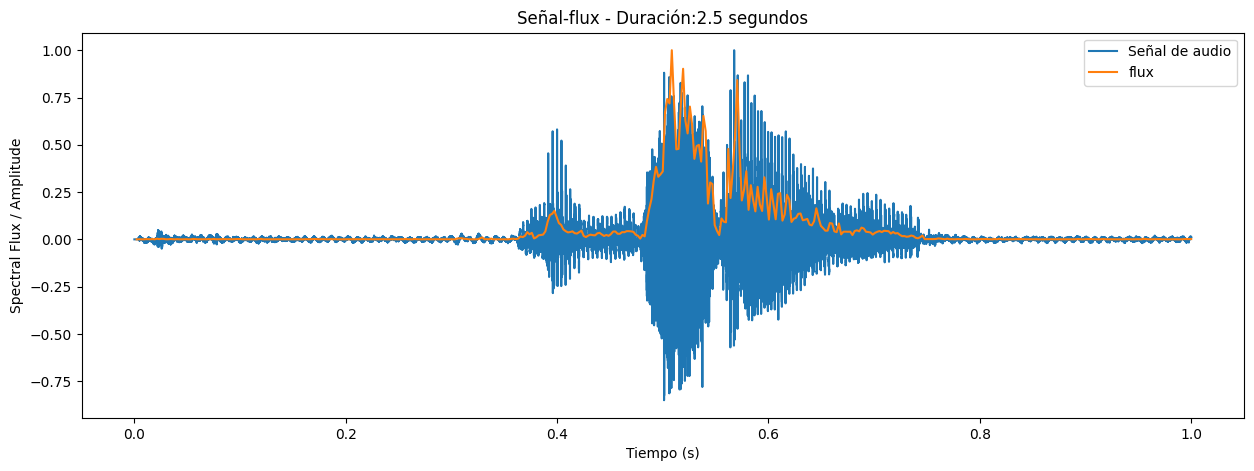
\includegraphics[width=0.8\linewidth]{trimming1.png}
    \caption{Flujo Espectral sobre la señal de Audio}
    \label{trimming 1}
\end{figure}

Para producir el recorte del audio con esta propiedad basta con definir un umbral y proceder. Sin embargo, este corte es sensible a ciertas perturbaciones en el audio que se presentan como picos iniciales y finales en la señal. En ese caso, hay que definir un umbral suficientemente grande de modo de pasar por alto esos picos. Al hacer eso, el audio queda recortado de más, eliminando partes del audio habladas en los extremos, como sucedería en el ejemplo que se muestra en la Figura ~\ref{trimming 2}.

\begin{figure}[h]
    \centering
    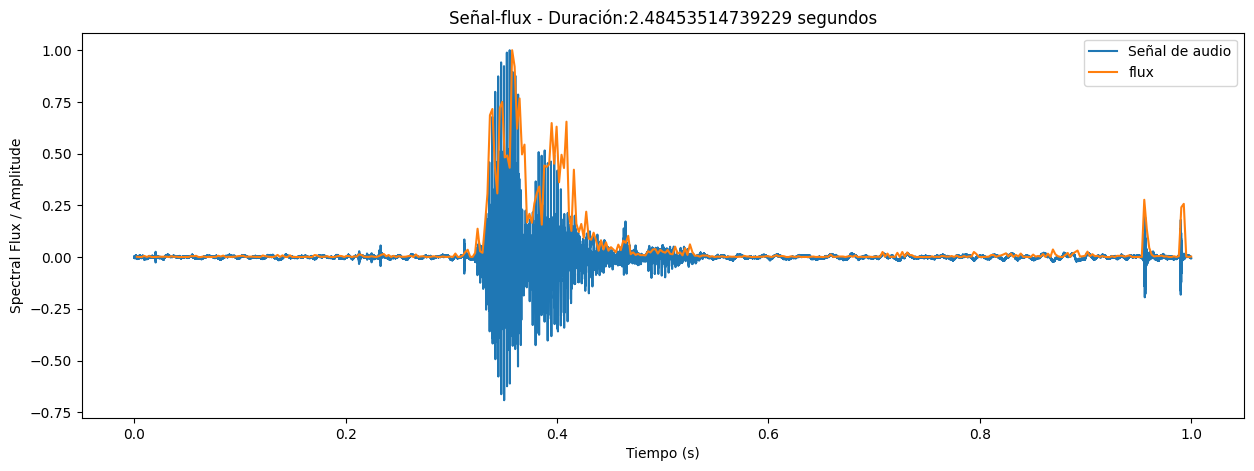
\includegraphics[width=0.8\linewidth]{trimming2.png}
    \caption{Flujo Espectral - Audios con Picos}
    \label{trimming 2}
\end{figure}

Como estrategia para resolver este problema, se propone definir un umbral mínimo y un umbral máximo. El umbral máximo debe ser tal que permita pasar por alto los picos, y luego el umbral mínmo sirve como ajuste fino del corte. De esa manera, se buscaría en la señal de flujo espectral el primer instante a la izquierda y a la derecha del audio en donde se supere el umbral, y desde ese punto y buscando hacia la izquierda en el extremo izquierdo o hacia la derecha en el extremo derecho encontrar el primer instante de tiempo en el que la señal de flujo espectral se encuentre por debajo del umbral máximo. El problema que se presenta en este caso es que existen audios en los que el flujo espectral es prácticamente nulo aún en partes habladas, como en el ejemplo de la Figura ~\ref{trimming 3}. Esto hace que el umbral míximo deba ser prácticamente igual a cero.

\begin{figure}[h]
    \centering
    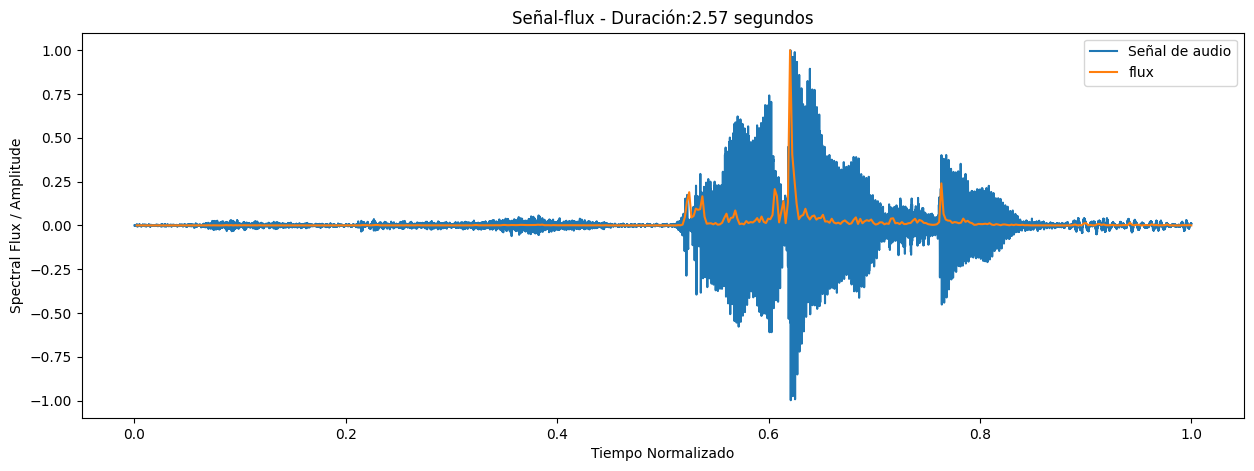
\includegraphics[width=0.8\linewidth]{trimming3.png}
    \caption{Flujo Espectral - Umbral mínimo}
    \label{trimming 3}
\end{figure}

Para resolver este problema, se introduce una segunda característica que sirve como envolvente de la señal original, que es el valor \textbf{RMS} de la señal. Este se calcula en frames a lo largo de la duración de la señal. Ahora, la estrategia es la misma, pero el umbral mínimo se define a partir de una fracción del valor RMS y no a partir de una fracción del valor del flujo espectral. En la Figura ~\ref{trimming 4} se muestra un ejemplo de este corte. En esa figura, la línea horizontal de color rojo indica el umbral de corte grueso por flujo espectral, mientras que la línea horizontal de color azul indica el umbral de corte fino por RMS. Las líneas punteadas verticales indican los puntos de corte, las rojas indican los puntos determinados por el corte grueso, mientras que las azules indican los puntos finales de corte fino por RMS. Como se puede observar, ahora es posible superar los picos finales que se presentan en la señal de audio.


\begin{figure}[h]
    \centering
    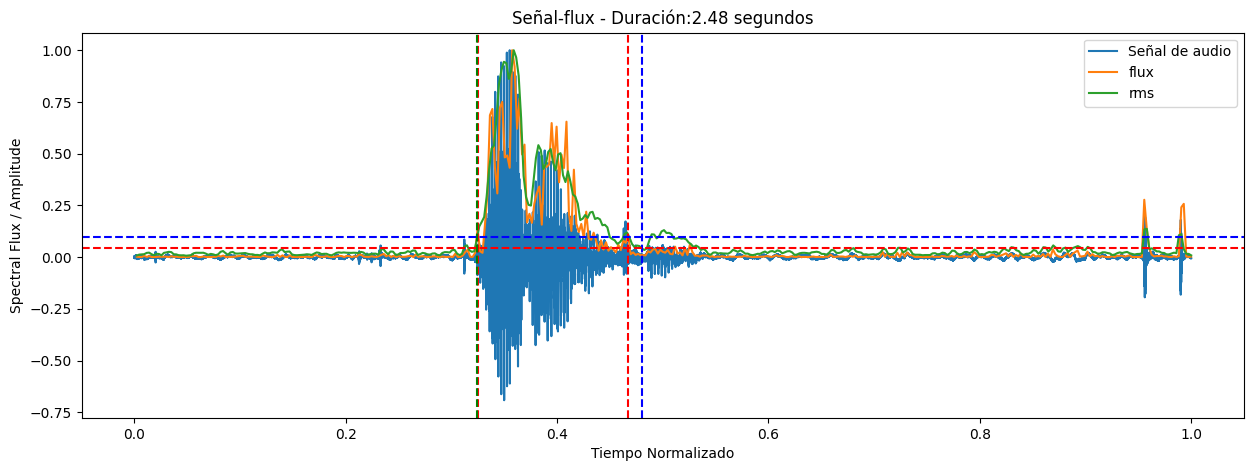
\includegraphics[width=0.8\linewidth]{trimming4.png}
    \caption{Flujo Espectral - RMS - Ejemplo de Corte}
    \label{trimming 4}
\end{figure}
%--------------------------------EXTRACCIÓN DE CARACTERÍSTICAS----------------------------
\subsubsection{Extracción de Características}
En las figuras de esta sección, en el eje \(X\) se representa la razón entre el valor RMS de las señales de audio y el valor máximo de la señal, mientras que en el eje \(Y\) se representa la característica de que se trate. Los colores de los puntos se corresponden con los colores de las frutas que representan.

La extracción de características comenzó con pruebas con los coeficientes de Mel, \textbf{MFCC} (Mel Frequency Cepstral Coefficients por sus siglas en inglés), dado que la investigación arrojó que los mismos son características ampliamente utilizadas en el reconocimiento de voz. Estos tienen la capacidad de describir los fonemas (unidades de sonido de un idioma) y toman en cuenta la percepción del oído humano al utilizar la escala logarítmica de Mel para la representación de características en función de la frecuencia.

En primer lugar, se probó utilizando la media de cada coeficiente de Mel a lo largo de la duración del audio, conservando aquellas componentes que producían la mayor contribución a la separación o que tenían la menor variación dentro de cada grupo. Varias otras pruebas se realizaron con los coeficientes de Mel, por nombrar otra, se probó la utilización de los valores de los mismos a lo largo de todo el audio dispuestos en un solo vector largo, para lo que se tuvo primero que normalizar los audios en amplitud y en duración sin lograr tampoco una separación y agrupamiento satisfactorio.

En el camino, se descubrió una técnica denominada Análisis de Componentes Principales, \textbf{PCA} (Principal Component Analysis, por sus siglas en inglés), que permite la reducción de un conjunto de k observaciones en un espacio m-dimensional a un conjunto de k observaciones en un espacio n-dimensional con n \textless\ m, conservando la mayor cantidad posible de variación a través de los datos, pero de modo tal que las componentes del nuevo espacio son linealmente independientes entre sí.

Al no obtener los resultados esperados haciendo uso solo de los MFCCs, es que se decidió hacer pruebas con otras medidas agregadas del audio, entre ellas \textbf{BER} (Band Energy Ratio, por sus siglas en inglés), \textbf{ZCR} (Zero Crossing Rate, por sus siglas en inglés), la envolvente del audio, etc.

A continuación, se detallan aquellas características que finalmente se utilizaron.

\begin{itemize}
    \item \textbf{BER:} Esta medida proporciona información sobre cómo está distribuida la energía en distintas partes del espectro de frecuencia. En esta solución se calcula como la fracción de la energía comprendida por debajo de cierta frecuencia de corte.
    \begin{itemize}
        \item \textbf{Máximo:} Se utiliza el máximo del BER para una frecuencia de corte de 600 Hz. En la Figura ~\ref{BER 1} se muestra cómo se puede lograr una separación de las peras respecto de los demás.
        \item \textbf{Mínimo:} Se utiliza el mínimo del BER a las frecuencias de corte de 1900, 5000 y 9000 Hz, en las Figuras~\ref{BER 2},~\ref{BER 3} y~\ref{BER 4}, respectivamente. Como se puede ver, la primera permite la separación de las peras respecto de los demás, la segunda logra una separación de las bananas respecto de las manzanas y la última una separación de las manzanas respecto de los demás, observándose cierta estratificación de los grupos en el medio.
        \item \textbf{Desviación estándar:} Para el BER normalizado y considerado respecto de la media. Se tomó con frecuencias de corte a 8000 Hz (Figura ~\ref{BER 5}) y 1000 Hz (Figura ~\ref{BER 6}). Se puede observar cómo en el primer caso se logra una separación de las manzanas respecto de los otros grupos mientras que en el segundo caso se logra una separación de las peras respecto de los otros grupos.
            \begin{figure}[htbp]
                \begin{minipage}[t]{0.5\textwidth}
                    \centering
                    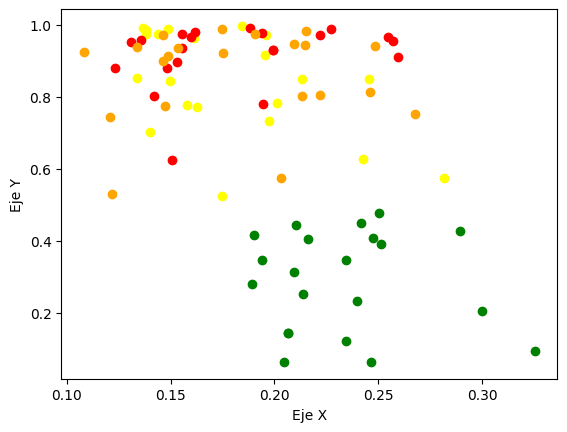
\includegraphics[width=0.8\linewidth]{BER1.png}
                    \caption{Máximo BER}
                    \label{BER 1}
                \end{minipage}%
                \begin{minipage}[t]{0.5\textwidth}
                    \centering
                    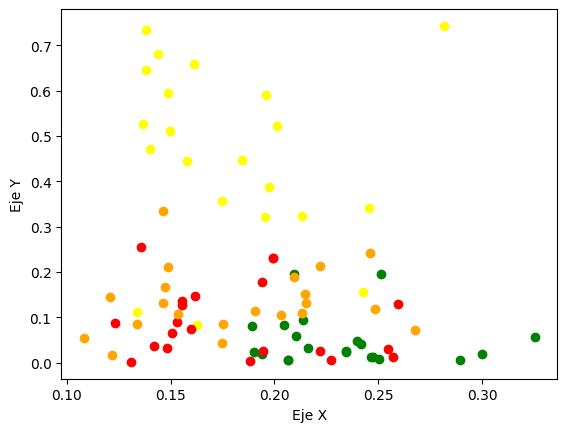
\includegraphics[width=0.8\linewidth]{BER2.png}
                    \caption{Mínimo BER - 1900 Hz}
                    \label{BER 2}
                \end{minipage}
            \end{figure}
            \begin{figure}[htbp]
                \begin{minipage}[t]{0.5\textwidth}
                    \centering
                    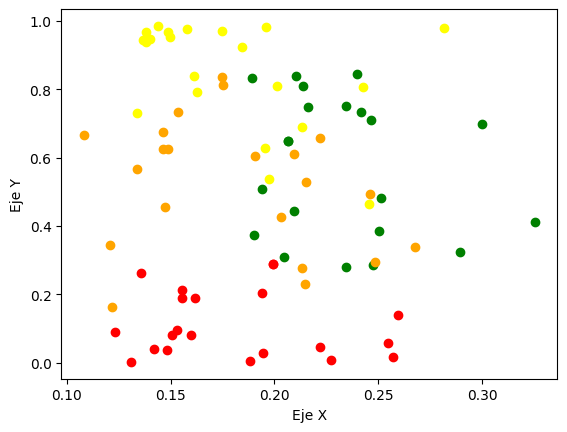
\includegraphics[width=0.8\linewidth]{BER3.png}
                    \caption{Mínimo BER - 5000 Hz}
                    \label{BER 3}
                \end{minipage}%
                \begin{minipage}[t]{0.5\textwidth}
                    \centering
                    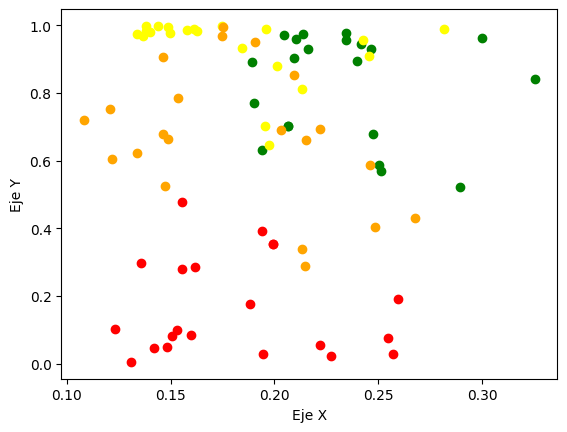
\includegraphics[width=0.8\linewidth]{BER4.png}
                    \caption{Mínimo BER - 9000 Hz}
                    \label{BER 4}
                \end{minipage}
            \end{figure}
            \begin{figure}[!htbp]
                \begin{minipage}[t]{0.5\textwidth}
                    \centering
                    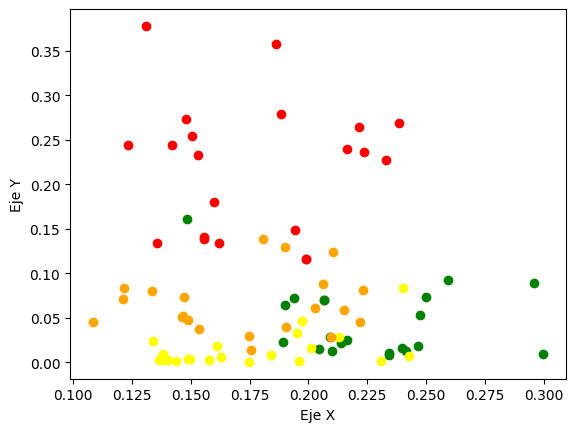
\includegraphics[width=0.8\linewidth]{BER5.png}
                    \caption{Std BER - 8000 Hz}
                    \label{BER 5}
                \end{minipage}%
                \begin{minipage}[t]{0.5\textwidth}
                    \centering
                    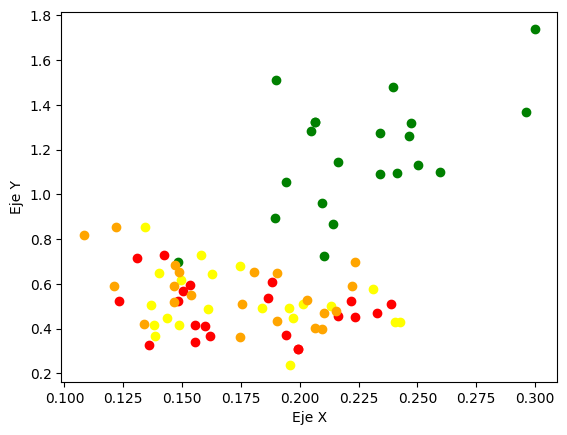
\includegraphics[width=0.8\linewidth]{BER6.png}
                    \caption{Std BER - 1000 Hz}
                    \label{BER 6}
                \end{minipage}
            \end{figure}
    \end{itemize}
    \item \textbf{Zero Crossing Rate (ZCR):} Esta medida cuenta la cantidad de veces que una señal cruza el eje horizontal (cero) en un intervalo de tiempo dado.    
        El ZCR expresa una tasa, representando la frecuencia con la que la señal cambia de polaridad. Un ZCR alto indica que la señal cambia de polaridad con frecuencia. Por otro lado, un ZCR bajo indica que la señal mantiene la misma polaridad durante un período de tiempo prolongado, lo que podría ser característico de señales más suaves.
    \begin{itemize}
        \item \textbf{Media:} Se obtiene respecto del valor máximo luego de un filtro pasa banda con corte en 1000 y 5000 Hz. Como se puede ver en la Figure~\ref{ZCR 1} esto logra la separación de las manzanas respecto de los demás grupos. Eso se debe a una variación de esta propiedad que no presentan el resto de los grupos cuando se pronuncia la letra 'z'.
            \begin{figure}[h]
                \centering
                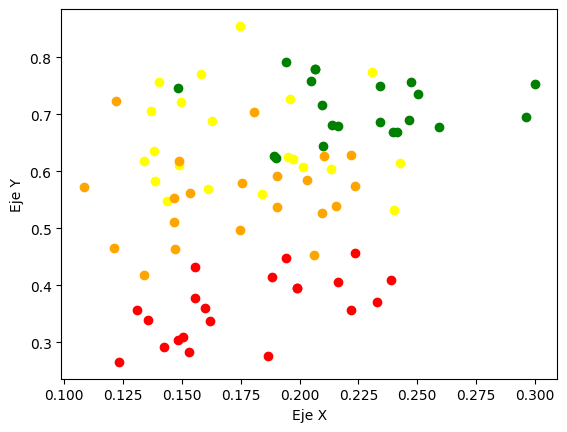
\includegraphics[width=0.4\linewidth]{ZCR1.png}
                \caption{Zero Crossing Rate - Media}
                \label{ZCR 1}
            \end{figure}
        \item \textbf{Máximo:} Se obtiene luego de un filtro pasa banda con cortes en 10 y 1000 Hz. En la Figura ~\ref{ZCR 2} se puede observar como nuevamente las manzanas se separan del resto de los grupos quedando las peras y las manzanas en grupos separados.
            \begin{figure}[h]
                \centering
                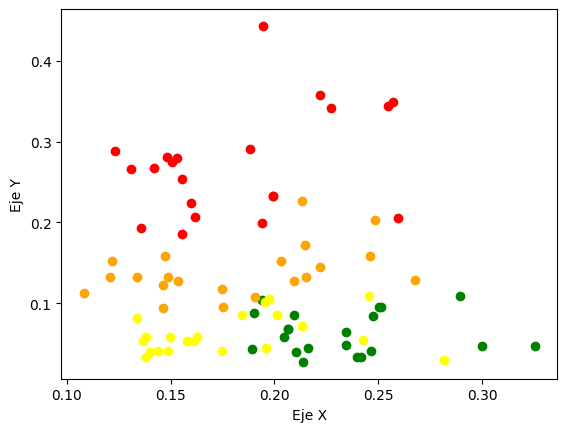
\includegraphics[width=0.4\linewidth]{ZCR2.png}
                \caption{Zero Crossing Rate - Máximo}
                \label{ZCR 2}
            \end{figure}
        \item \textbf{Desviación Estándar:} Se obtiene respecto de la media luego de un filtro pasa banda con cortes en 20 y 10000 Hz. En la figura ~\ref{ZCR 3} se puede ver cómo las manzanas se separan del resto y en el centro se pueden observar un grupo casi solo de naranjas.
            \begin{figure}[h]
                \centering
                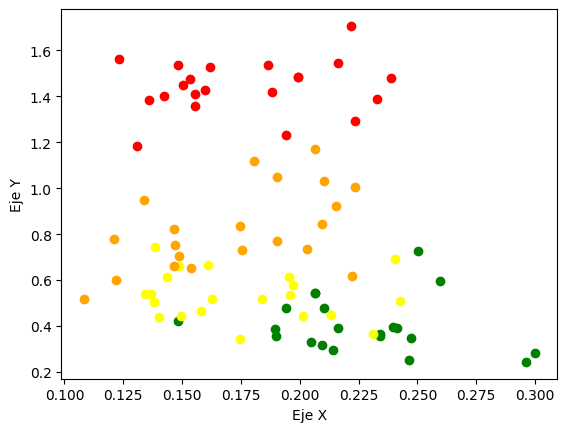
\includegraphics[width=0.4\linewidth]{ZCR3.png}
                \caption{Zero Crossing Rate - Desviación Estándar}
                \label{ZCR 3}
            \end{figure}
        \item \textbf{Media a 3/14:} Luego de un filtro pasabanda con cortes en 1000 y 5000 Hz se calcula la media del audio normalizado en ese punto en la duración del audio a lo largo de 10 frames, 5 a cada lado. Nuevamente se observa una separación de las manzanas (Figure ~\ref{ZCR 4})
            \begin{figure}[h]
                \centering
                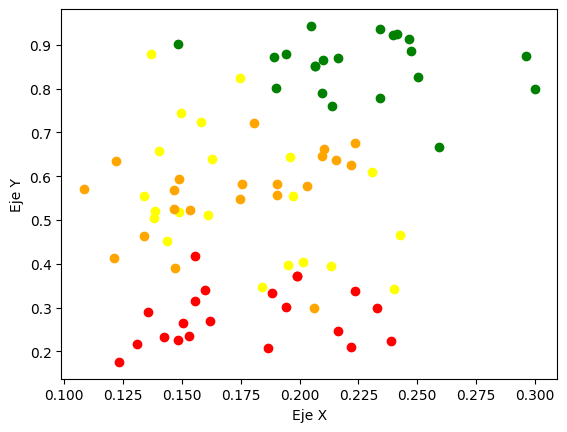
\includegraphics[width=0.4\linewidth]{ZCR4.png}
                \caption{Zero Crossing Rate - Media a 3/14}
                \label{ZCR 4}
            \end{figure}
        \item \textbf{Máximo a 3/4:} Luego de un filtro pasabanda con cortes en 10 y 10000 Hz se calcula el máximo en ese punto en la duración del audio a lo largo de 20 frames, 10 a cada lado buscando resaltar las diferencias entre las naranjas y las demás frutas cuando se pronuncia la letra 'j' (Figura ~\ref{ZCR 4}).
            \begin{figure}[!h]
                \centering
                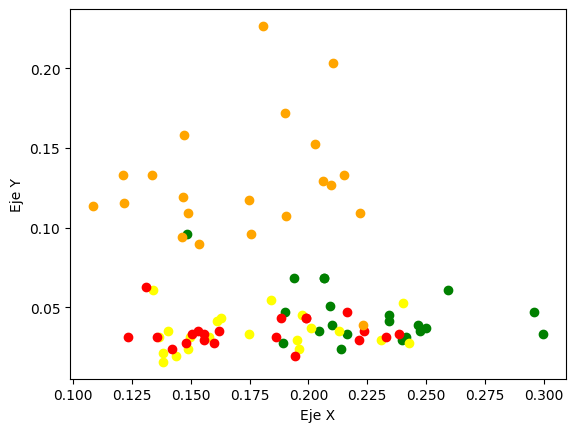
\includegraphics[width=0.4\linewidth]{ZCR5.png}
                \caption{Zero Crossing Rate - Máximo a 3/4}
                \label{ZCR 5}
            \end{figure}
    \end{itemize}
    \item \textbf{Spectral Roll Off:} El \textit{Spectral Roll-off} es una medida que indica la frecuencia por debajo de la cual se encuentra un cierto porcentaje de la energía total del espectro. Un valor bajo indica una concentración en frecuencias bajas, mientras que un valor alto implica una distribución hacia frecuencias más altas.
    \begin{itemize}
        \item \textbf{Media:} Se obtiene respecto del máximo luego de un filtro pasa banda con cortes en 100 y 8500 considerando un pocentaje del 28\% de la energía del espectro. Se separan las manzanas y las peras también las naranjas de las bananas y de las peras aunque queda un solapamiento entre bananas y naranjas (Figura ~\ref{SRO 1}).
        \begin{figure}[h]
            \centering
            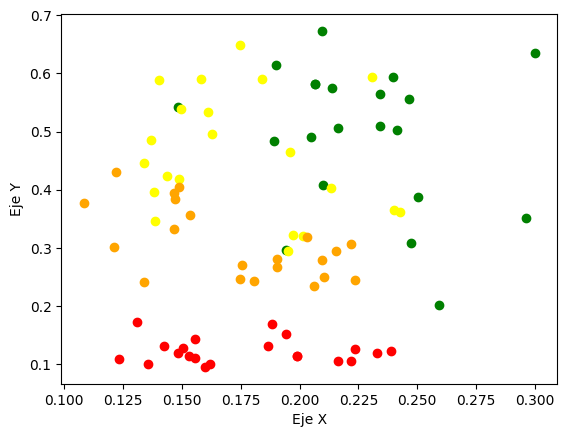
\includegraphics[width=0.4\linewidth]{SRO1.png}
            \caption{Spectral Roll Off - Media}
            \label{SRO 1}
        \end{figure}
        \item \textbf{Máximo:} Se obtiene luego de un filtro pasa banda con cortes en 100 y 8500 considerando un pocentaje del 55\% de la energía del espectro. Se observa una separación de las manzanas (Figura ~\ref{SRO 2}).
        \begin{figure}[h]
            \centering
            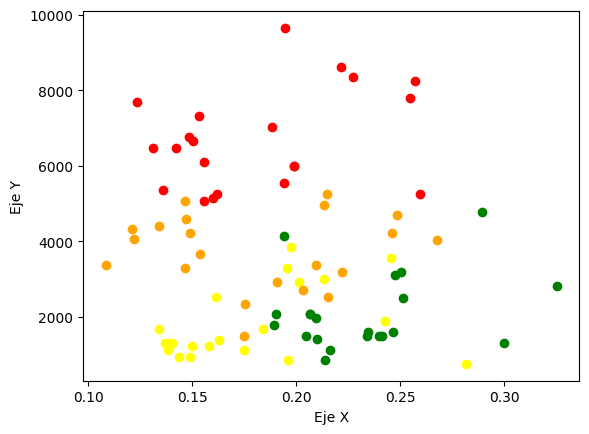
\includegraphics[width=0.4\linewidth]{SRO2.png}
            \caption{Spectral Roll Off - Máximo}
            \label{SRO 2}
        \end{figure}
        \item \textbf{Desviación Estándar:} Se obtiene respectro de la media luego de un filtro pasa banda con cortes en 50 y 8500 considerando un pocentaje del 28\% de la energía del espectro. Nuevamente se observa una separación de las manzanas (Figura ~\ref{SRO 3}).
        \begin{figure}[h]
            \centering
            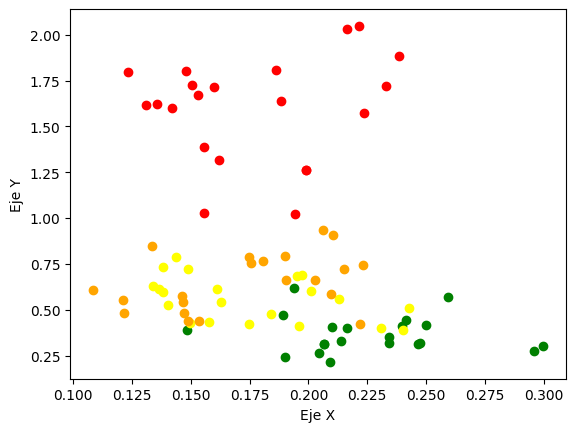
\includegraphics[width=0.4\linewidth]{SRO3.png}
            \caption{Spectral Roll Off - Desviación Estándar}
            \label{SRO 3}
        \end{figure}
    \end{itemize}
    \item \textbf{MFCCs:} Como ya se mencionó, es de las principales características utilizadas para el reconocimiento de voz dado que tiene la capacidad de identificar fonemas y demás.
    \begin{itemize}
        \item \textbf{Máximo del coeficiente 3:} Se obtiene luego de un filtro pasa banda con cortes en 500 y 5000. Se separan las manzanas (Figura ~\ref{MFCCS 1}).
        \begin{figure}[h]
            \centering
            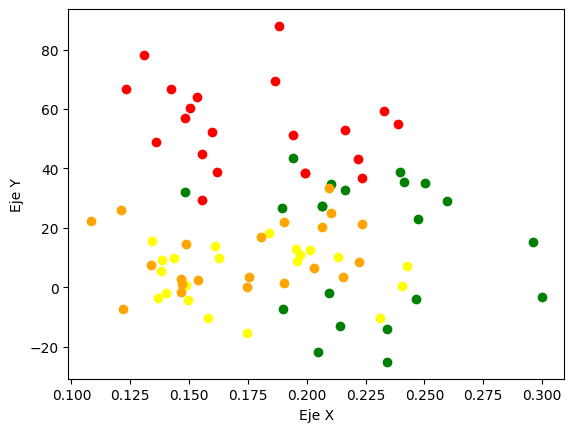
\includegraphics[width=0.4\linewidth]{MFCCS1.png}
            \caption{MFCCs - Máximo del coeficiente 3}
            \label{MFCCS 1}
        \end{figure}
        \item \textbf{Desviación estándar coeficiente 1 a 4/5:} Se obtiene respecto de la media luego de un filtro pasa banda con cortes en 10 y 8000 en 20 frames alrededor de este punto en la duración del audio (10 frames de cada lado). Aunque existe cierta dispersión, se observa una separación de las naranjas (Figura ~\ref{MFCCS 3}).
        \begin{figure}[!h]
            \centering
            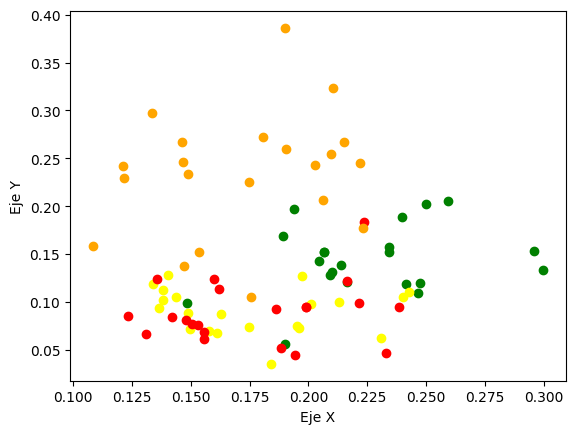
\includegraphics[width=0.4\linewidth]{MFCCS3.png}
            \caption{MFCCs - Desviación estándar coeficiente 1 a 4/5}
            \label{MFCCS 3}
        \end{figure}
    \end{itemize}
    \item \textbf{Envolvente:} El cálculo del valor RMS en cada frame en que se divide un audio funciona como una buena envolvente de amplitud de la señal. De esta envolvente se toman 30 componentes equi-espaciadas de las cuales se conservan la componente 11 y la 12 (Figura~\ref{ENVELOPE}). Dentro de todo se logra una separación de las manzanas respecto al resto
    \begin{figure}[h]
        \centering
        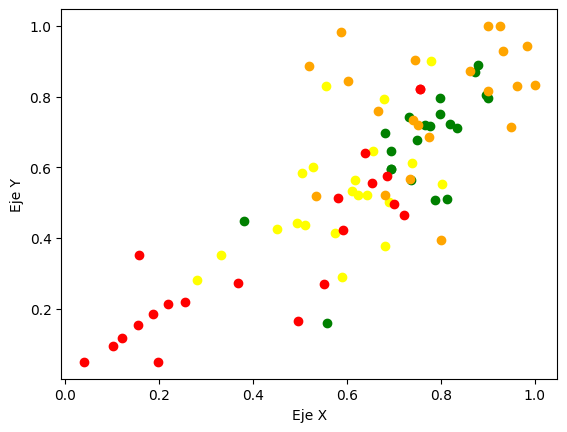
\includegraphics[width=0.4\linewidth]{ENVELOPE.png}
        \caption{Envolvente componentes 11 y 12}
        \label{ENVELOPE}
    \end{figure}
\end{itemize}
Como se puede notar, algunas de las características extraídas son demasiado específicas. Sin embargo, este conjunto de características fue seleccionado después de muchas pruebas, ya que se consideró que lograba los mejores resultados en términos de agrupamiento y separación.

\subsubsection{Reducción de componentes}
La cantidad de componentes del vector de características de cada audio es de 17. Se pretende hacer la visualización en un gráfico de los agrupamientos que se consiguen, y para eso, luego de la extracción de las características de los audios se utiliza PCA para reducir el conjunto de componentes a 3. En la Figuras~\ref{GRUPOS 1} y ~\ref{GRUPOS 2} se observa el agrupamiento conseguido.
\begin{figure}[!htbp]
    \centering
    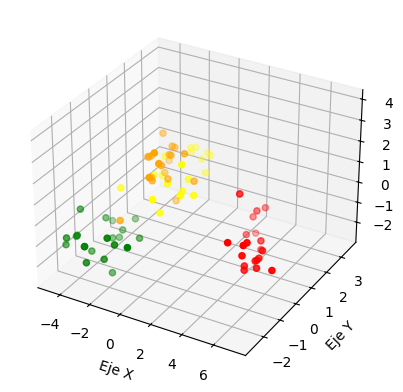
\includegraphics[width=0.6\linewidth]{GRUPOS1.png}
    \caption{Agrupamiento post PCA - 1}
    \label{GRUPOS 1}
\end{figure}
\begin{figure}[!htbp]
    \centering
    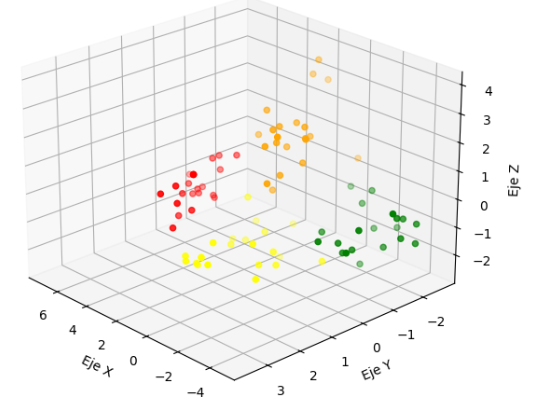
\includegraphics[width=0.6\linewidth]{GRUPOS2.png}
    \caption{Agrupamiento post PCA - 2}
    \label{GRUPOS 2}
\end{figure}
\newpage
\subsection{Reconocimiento de Imágenes}
\subsubsection{Separación del fondo}

Para lograr la separación de la fruta del fondo se exploraron diversas alternativas. A continuación, se describe brevemente el proceso indicando los resultados o los pasos de las partes que quedaron en la solución final.

Principalmente, el problema se abordó tratando de que las imágenes pudieran ser tomadas en diferentes tipos de fondos y no en uno solo normalizado, para que, por ejemplo, sea posible sacar la foto de la fruta sobre una mesa de cualquier tipo. Siguiendo esta línea, lo primero que se exploró fue la detección de contornos utilizando filtros de Sobel~\cite{sobel} (figure ~\ref{SOBEL}), sin embargo, esto también detectaba las diferentes texturas que podía llegar a tener el fondo, con lo cual no era una solución viable, ya que no se encontraba forma de separar el contorno de la fruta del resto de los contornos.
\begin{figure}[!htbp]
    \centering
    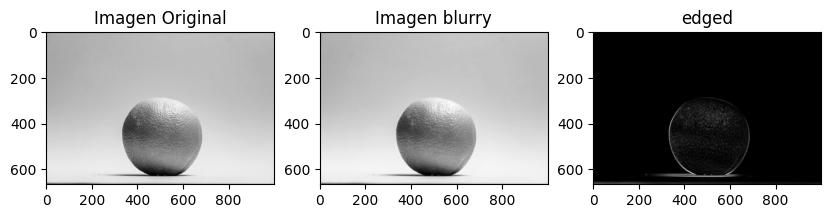
\includegraphics[width=0.6\linewidth]{SOBEL.png}
    \caption{Ejemplo de aplicación de filtros de Sobel}
    \label{SOBEL}
\end{figure}
Entonces, se exploró el uso de máscaras de color que pudieran detectar cualquiera de los colores de las frutas que se consideran (naranja, verde, amarillo y rojo). Estas máscaras se diseñan en el espacio de colores HSV (Hue, Saturation, Value por sus siglas en inglés), que es una escala cómoda para el manejo de colores, dado que distribuye distintos colores en un cilindro en el que el color varía según el ángulo, la iluminación en la altura y la saturación o pureza del color en el radio, permitiendo pasar de forma continua por todo el rango de lo que se puede llegar a considerar rojo, por poner un ejemplo. El inconveniente se presentaba en estos casos cuando el fondo tenía colores parecidos a los mencionados, dado que quedaban incluidos dentro de lo que se consideraba como fruta.

Por este motivo, se comenzó un trabajo de pruebas de distintas máscaras para evaluar el comportamiento de las mismas. Las máscaras se construían considerando canales de distintas representaciones de la imagen. Por ejemplo, se consideraba el canal H del espacio HSV y se aplicaba binarización (pasar a blanco y negro) haciendo uso de OTSU~\cite{otsu}. Esto se practicó con los canales L, A, B del espacio LAB~\cite{lab}, con los canales H, S y V, con los canales R, G B y con la imagen en escala de grises. En la figura~\ref{MASCARAS} se muestra un ejemplo de esto. En la misma, la máscara la máscara señalada como kmeans es una máscara obtenida de aplicar el algoritmo kmeans con dos clusters y en el que los datos a segmentar son los vectores que tienen los valores HSV, LAB, RGB y de escala de grises y hay tantos datos como pixeles de la imágen. Está máscara como se puede ver funciona bastante bien para la separación d ela fruta aunque se puede comprobar que no funciona de forma perfecta en todos los casos. La máscara indicada como color es la máscara obtenida por la detección de colores antes mencionada.

\begin{figure}[!htbp]
    \centering
    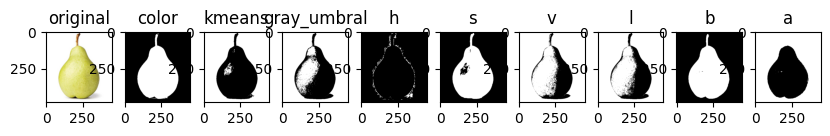
\includegraphics[width=\linewidth]{MASCARAS.png}
    \caption{Máscaras probadas}
    \label{MASCARAS}
\end{figure}

Lo que se puede observar que sucede es que los fondos de las máscaras, en algunas de las ocasiones, son negros y en otros son blancos. En lugar de tomar las máscaras en sí, lo que se buscó es, con Sobel, los contornos y luego se volvió a binarizar con OTSU para resaltar solamente los contornos, como se muestra en la imagen~\ref{CONTORNOS} lo que permite pasar por alto la situación de qué color queda en el fondo. En esa imágen Whole representa la combinación de todos los contornos de las máscaras. Esta figura muestra que son varias las máscaras que pueden funcionar adecuadamente para separar a la fruta del fondo. Esto es sin embargo para frutas en las que el fondo de la imagen original es blanco o de otro color pero de tipo uniforme y sin texturas. En fondos mas complejos como por ejemplo, en una mesa con cierta textura, en cambio, en general no hay siquiera una máscara que permita separar correctamente a la fruta del fondo

\begin{figure}[!htbp]
    \centering
    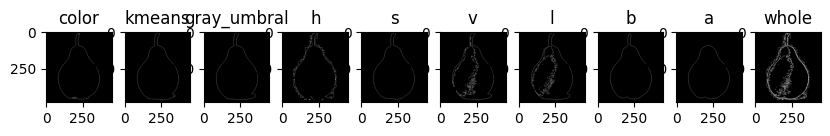
\includegraphics[width=\linewidth]{CONTORNOS.png}
    \caption{Contornos de las máscaras}
    \label{CONTORNOS}
\end{figure}

Esta figura muestra que son varias las máscaras que pueden funcionar adecuadamente para separar a la fruta del fondo. Esto es sin embargo para frutas en las que el fondo de la imagen original es blanco o de otro color pero de tipo uniforme y sin texturas. En fondos mas complejos como por ejemplo, en una mesa con cierta textura, en cambio, en general no hay siquiera una máscara que permita separar correctamente a la fruta del fondo.

Por esos motivos, finalmente se decidió utilizar solamente fondos blancos en las imágenes y se simplificó la separación de la fruta respecto del fondo.

El procesamiento final que se realiza en todas las imágenes para obtener las máscaras consiste en obtener los canales B del RGB, el canal S del espacio HSV y los canales A y B del espacio LAB, ya que se consideró que con estos se conseguían las máscaras más inertes ante sombras o variaciones de iluminación del entorno. Con esos datos por píxel, se procede a realizar la segmentación en dos clusters utilizando Kmeans de la biblioteca `sklearn.cluster` (ver código). Lo que sucede con Kmeans es que, en ocasiones, el fondo de la máscara obtenida por segmentación puede ser blanco o negro; sin embargo, lo que se pretende es un fondo negro en todos los casos, con la parte de la imagen donde se encuentra la fruta en blanco. Esto se resolvió evaluando los colores de los píxeles (blanco o negro) de la máscara en las esquinas y en las aristas, en matrices de píxeles con tamaños iguales a la 20-ava parte de la menor dimensión de la imagen. Luego, contando la cantidad de píxeles del total que se encuentran en blanco, se puede determinar si el fondo de la máscara es blanco o negro. Si la cantidad es mayor al 75\%, como quedó fijado, se considera que es fondo blanco y, por lo tanto, se invierte.

Con la máscara así definida, todavía se presentan algunos defectos, por los cuales existen zonas en los bordes de la fruta en los que hay varias zonas pequeñas aisladas blancas, principalmente debido a los reflejos de la iluminación y la presencia de sombras. Para resolver esto, se aplican operaciones de erosión para limpiar la imagen y luego una operación de dilatación para expandir la máscara en la zona de la fruta y unir todos los bordes irregulares. De esta máscara resultante, se obtiene el contorno con la función incorporada en la librería OpenCV. Este contorno luego se aproxima con líneas poligonales y se dibuja sobre una plantilla de fondo negro con relleno, de modo que todo en el interior del contorno es blanco y el exterior es negro. Esta es la máscara final que se aplicará posteriormente a la imagen para extraer las características y se guarda en un archivo.

En la figuras ~\ref{imagen ejemplo mascara} y ~\ref{mascara ejemplo mascara} se presentan como ejemplo una imágen y su máscara respectivamente.
\begin{figure}[!htbp]
    \begin{minipage}[t]{0.5\textwidth}
        \centering
        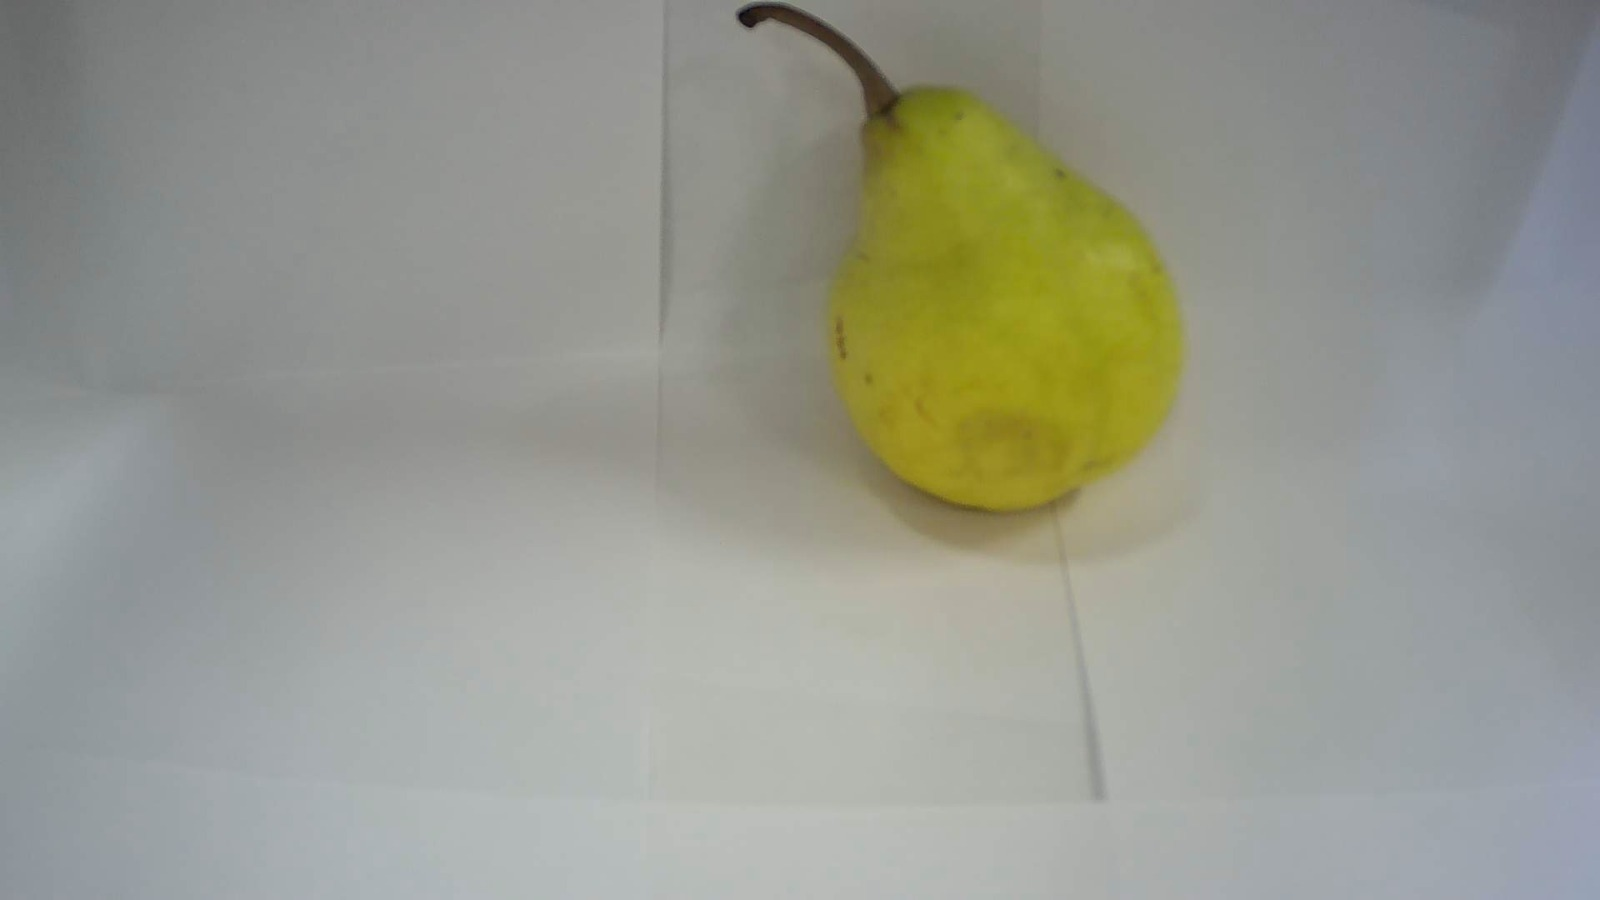
\includegraphics[width=0.8\linewidth]{imagen_mascara.jpeg}
        \caption{Imágen Ejemplo}
        \label{imagen ejemplo mascara}
    \end{minipage}%
    \begin{minipage}[t]{0.5\textwidth}
        \centering
        
\includegraphics[width=0.8\linewidth]{mascara_mascara.jpeg}
        \caption{Máscara Ejemplo}
        \label{mascara ejemplo mascara}
    \end{minipage}
\end{figure}

\subsection{Extracción de Características}


\end{document}